\documentclass{beamer}
%
% Choose how your presentation looks.
%
% For more themes, color themes and font themes, see:
% http://deic.uab.es/~iblanes/beamer_gallery/index_by_theme.html
%
\mode<presentation>
{
  \usetheme{Madrid}      % or try Darmstadt, Madrid, Warsaw, ...
  \usecolortheme{beaver} % or try albatross, beaver, crane, ...
  \usefonttheme{serif}  % or try serif, structurebold, ...
  \setbeamertemplate{navigation symbols}{}
  \setbeamertemplate{caption}[numbered]
} 

\usepackage{hyperref}
\usepackage[english]{babel}
\usepackage[utf8x]{inputenc}
\usepackage{pdfpages}
\usepackage{framed, color}
\definecolor{shadecolor}{rgb}{1,0.8,0.3}
\usepackage{color}

\definecolor{pblue}{rgb}{0.13,0.13,1}
\definecolor{pgreen}{rgb}{0,0.5,0}
\definecolor{pred}{rgb}{0.9,0,0}
\definecolor{pgrey}{rgb}{0.46,0.45,0.48}

\usepackage{listings}
\lstset{language=Python,
  showspaces=false,
  showtabs=false,
  breaklines=true,
  showstringspaces=false,
  breakatwhitespace=true,
  commentstyle=\color{pgreen},
  keywordstyle=\color{pblue},
  numbers=left,
  numbersep=5pt, 
  stringstyle=\color{pred},
  basicstyle=\ttfamily,
  frame=lrbt,xleftmargin=\fboxsep,xrightmargin=-\fboxsep
}

\title[Ragazze Digitali 2019]{Ragazze Digitali A.A. 2018/2019}
\author{E. Salvucci - S. Gattucci - C. Varini}
\date{}

\AtBeginSection[]
{
  \begin{frame}<beamer>
    \frametitle{Outline}
    \tableofcontents[currentsection,currentsubsection]
  \end{frame}
}

\begin{document}


\setbeamertemplate{background}
{
\includegraphics[width=\paperwidth,height=\paperheight]{images/ragazze_digitali.jpg}}
\begin{frame}
\mbox{}
\vspace{70.0mm}
\begin{center}
\href{https://github.com/ragazzedigitalicesena/slide-2019}{https://github.com/ragazzedigitalicesena/slide-2019}    
\end{center}

\end{frame}

\setbeamertemplate{background}{}

\begin{frame}{Alcune regole..}
	\begin{itemize}
	    \item Mano alzata
    \end{itemize}
\end{frame}

\begin{frame}{Alcune regole..}
	\begin{itemize}
	    \item Mano alzata
        \item Si Copia!
    \end{itemize}
\end{frame}

\begin{frame}{Alcune regole..}
	\begin{itemize}
	    \item Mano alzata
        \item Si Copia!
        \item Divertirsi!
    \end{itemize}
\end{frame}

\begin{frame}{Che cos'è la Scienza}
    
\footnote{Traduzione dalle slides del Prof. Andrea Omicini, Sistemi Distribuiti AA 18/19}
\begin{block}{Da: The Science Council}
\small{\url{http://sciencecouncil.org/about-us/our-definition-of-science/}}
% Science  is  the  pursuit  and  application  of  knowledge  and  understanding  of  the  natural  and  social  world  following  a  systematic methodology based on evidence
\vspace{0.5cm}

La Scienza è la ricerca e l'applicazione della conoscenza e della comprensione dei fenomeni naturali e sociali, che avviene seguendo una metodologia sistematica basata sui fatti.
\end{block}

\end{frame}

\begin{frame}{Che cos'è la Scienza}
    
\begin{block}{Da: The Science Council}
\small{\url{http://sciencecouncil.org/about-us/our-definition-of-science/}}
\vspace{0.5cm}

La Scienza è la ricerca e l'applicazione della conoscenza [..] seguendo una metodologia sistematica [...]
% In inglese "informatica" si dice Computer Science, quindi in questa settimana noi saremo scienziati (utilizzando i computer)
\end{block}

\end{frame}

\setbeamertemplate{background}
% Python
{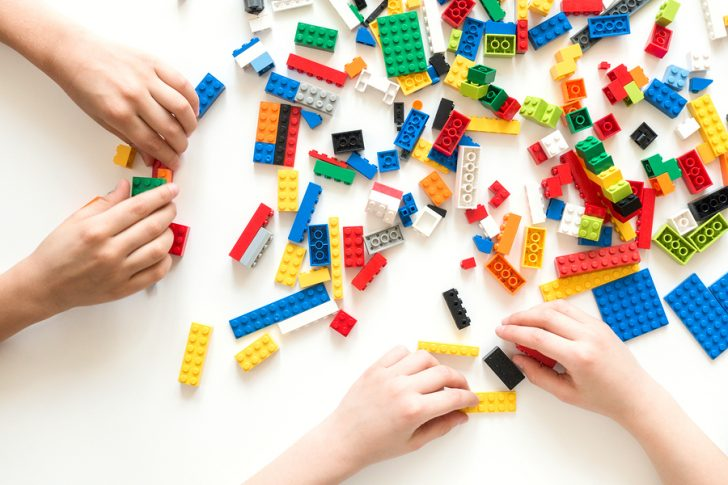
\includegraphics[width=\paperwidth,height=\paperheight]{images/lego.jpg}}
\begin{frame}{Cosa faremo}
\end{frame}

\setbeamertemplate{background}{}

\begin{frame}{Python}
    \begin{block}{Italiano}
        Ciao Mondo!
    \end{block}

    \begin{block}{Inglese}
        Hello World!
    \end{block}

    \begin{block}{Python}
        print "Hello World!"
    \end{block}
    
    \small{Faremo riferimento a questo libro, potete scaricarlo legalmente gratis
    \url{https://inventwithpython.com/invent4thed/}}

\end{frame}

\setbeamertemplate{background}
% Python
{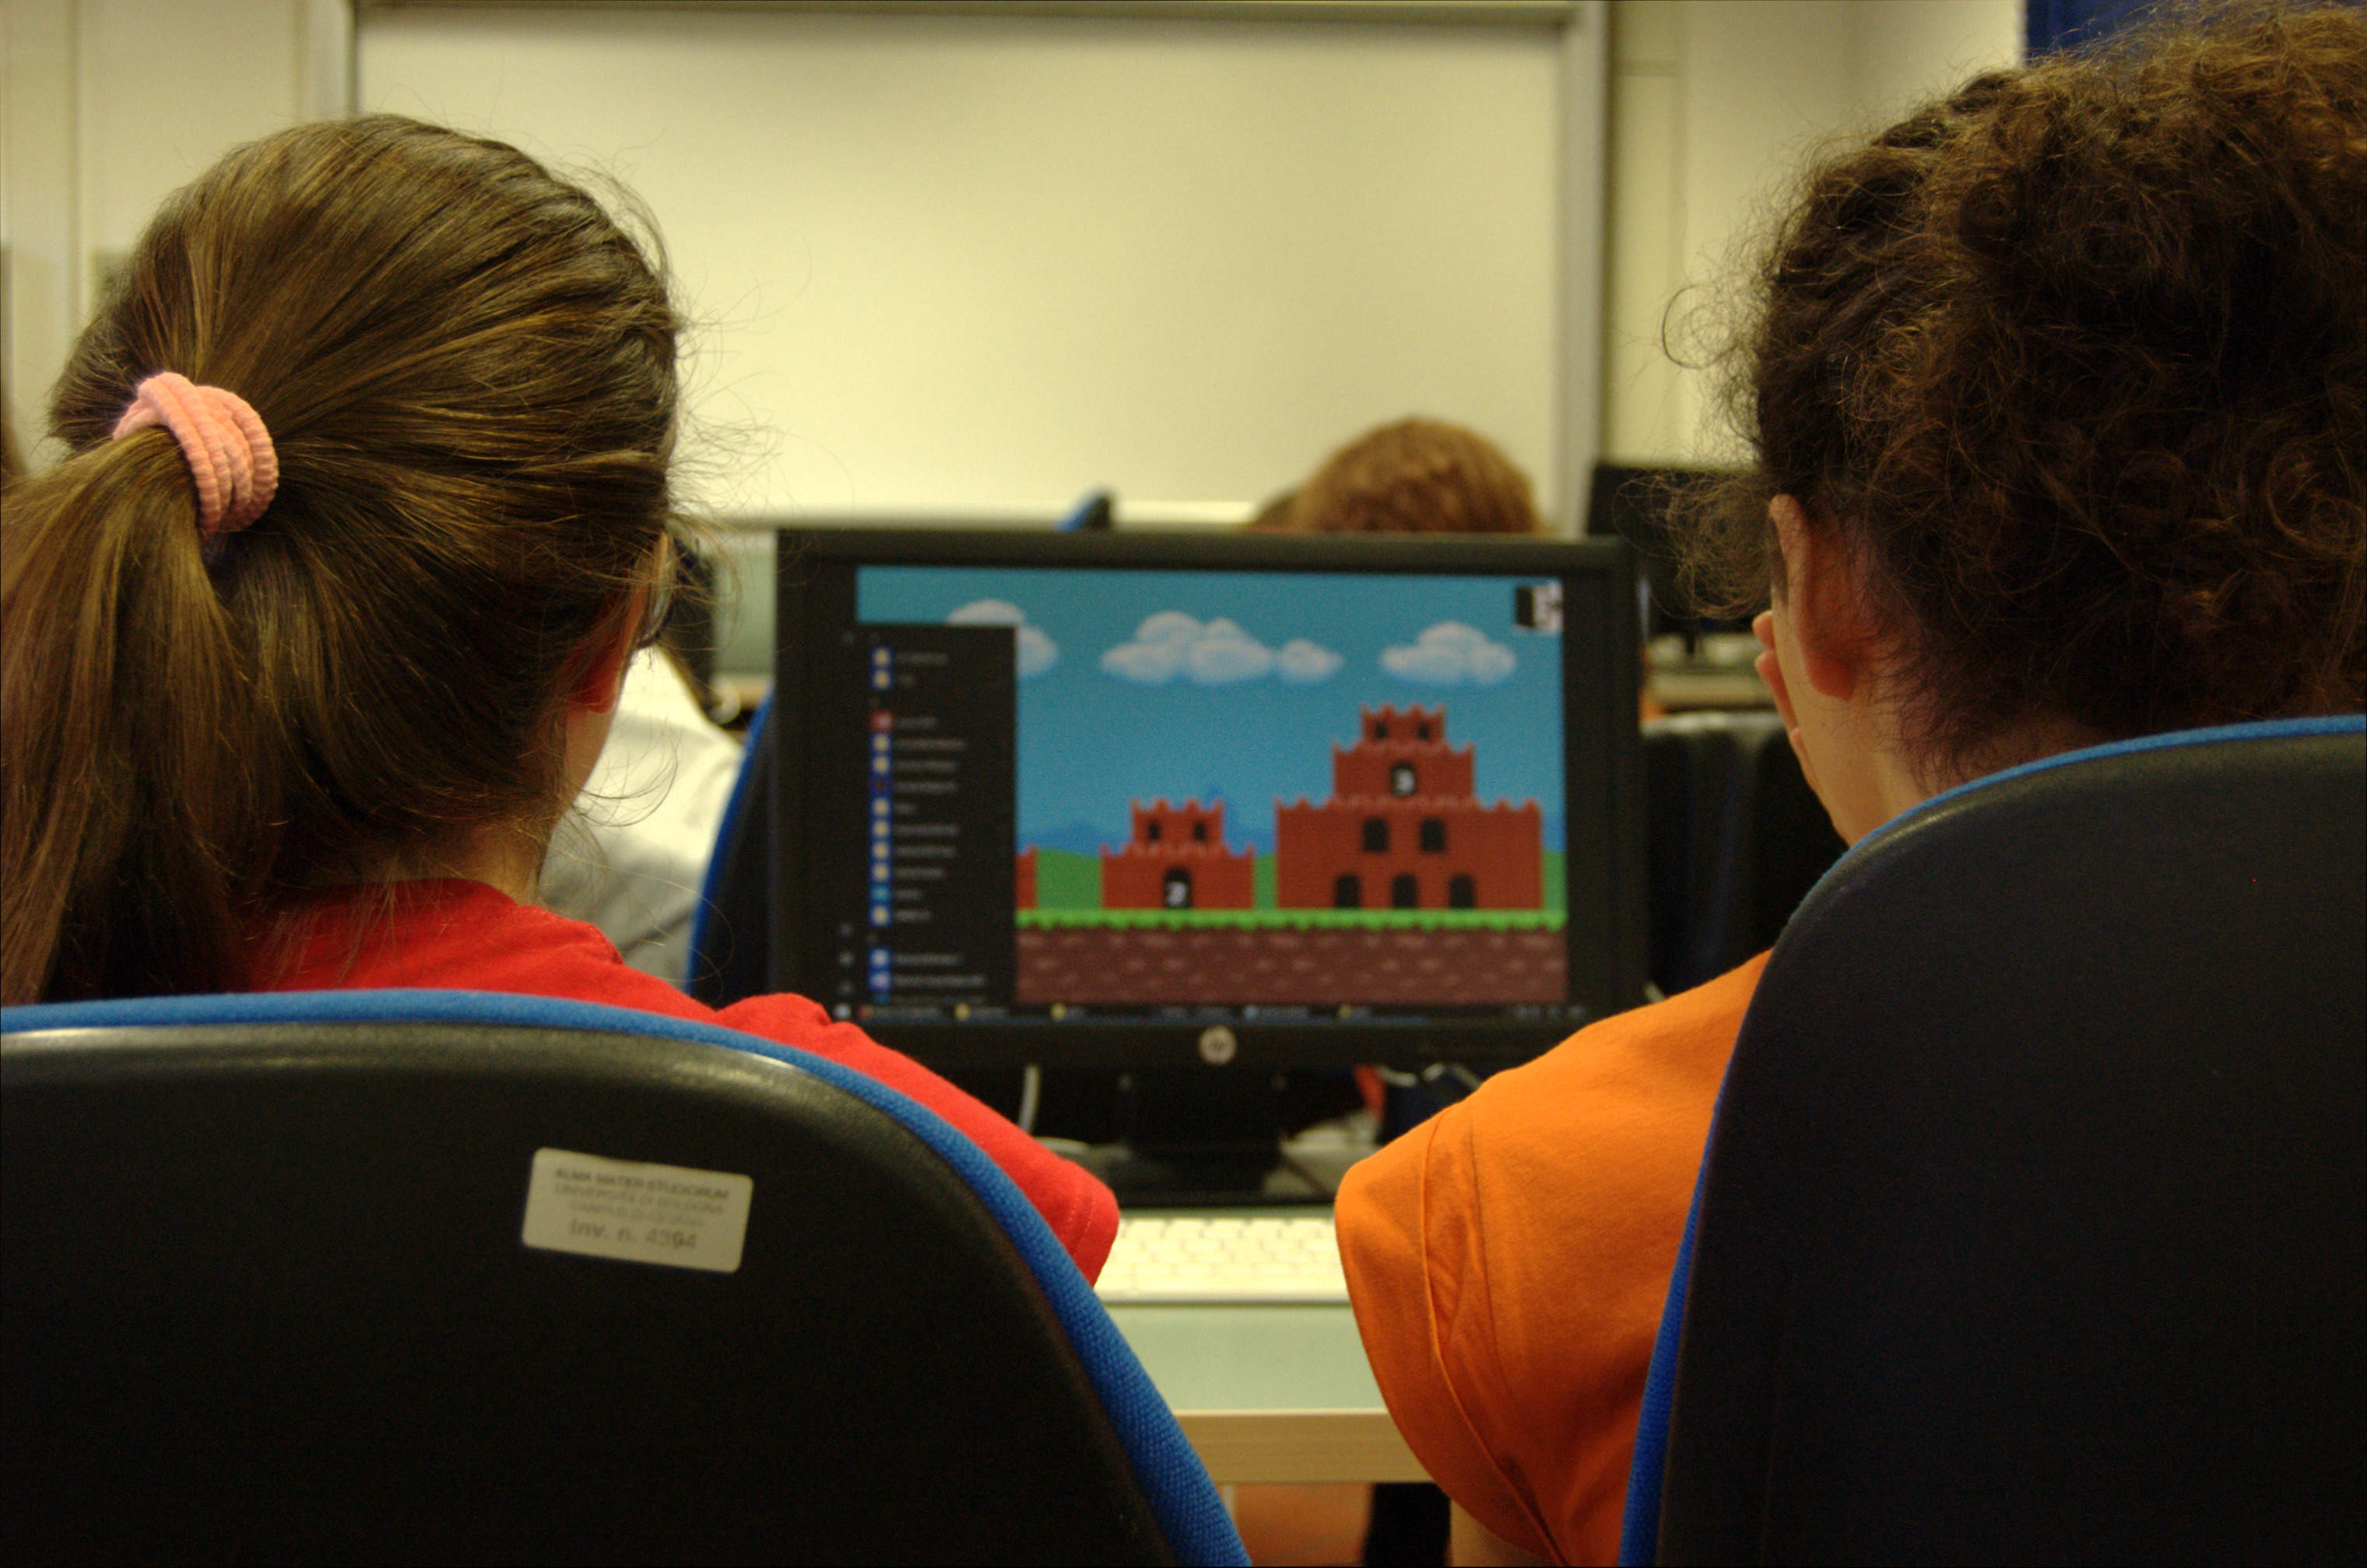
\includegraphics[width=\paperwidth,height=\paperheight]{images/summer_camp_2018_10.jpg}}
\begin{frame}{Cosa faremo}
\end{frame}

\setbeamertemplate{background}
% Python
{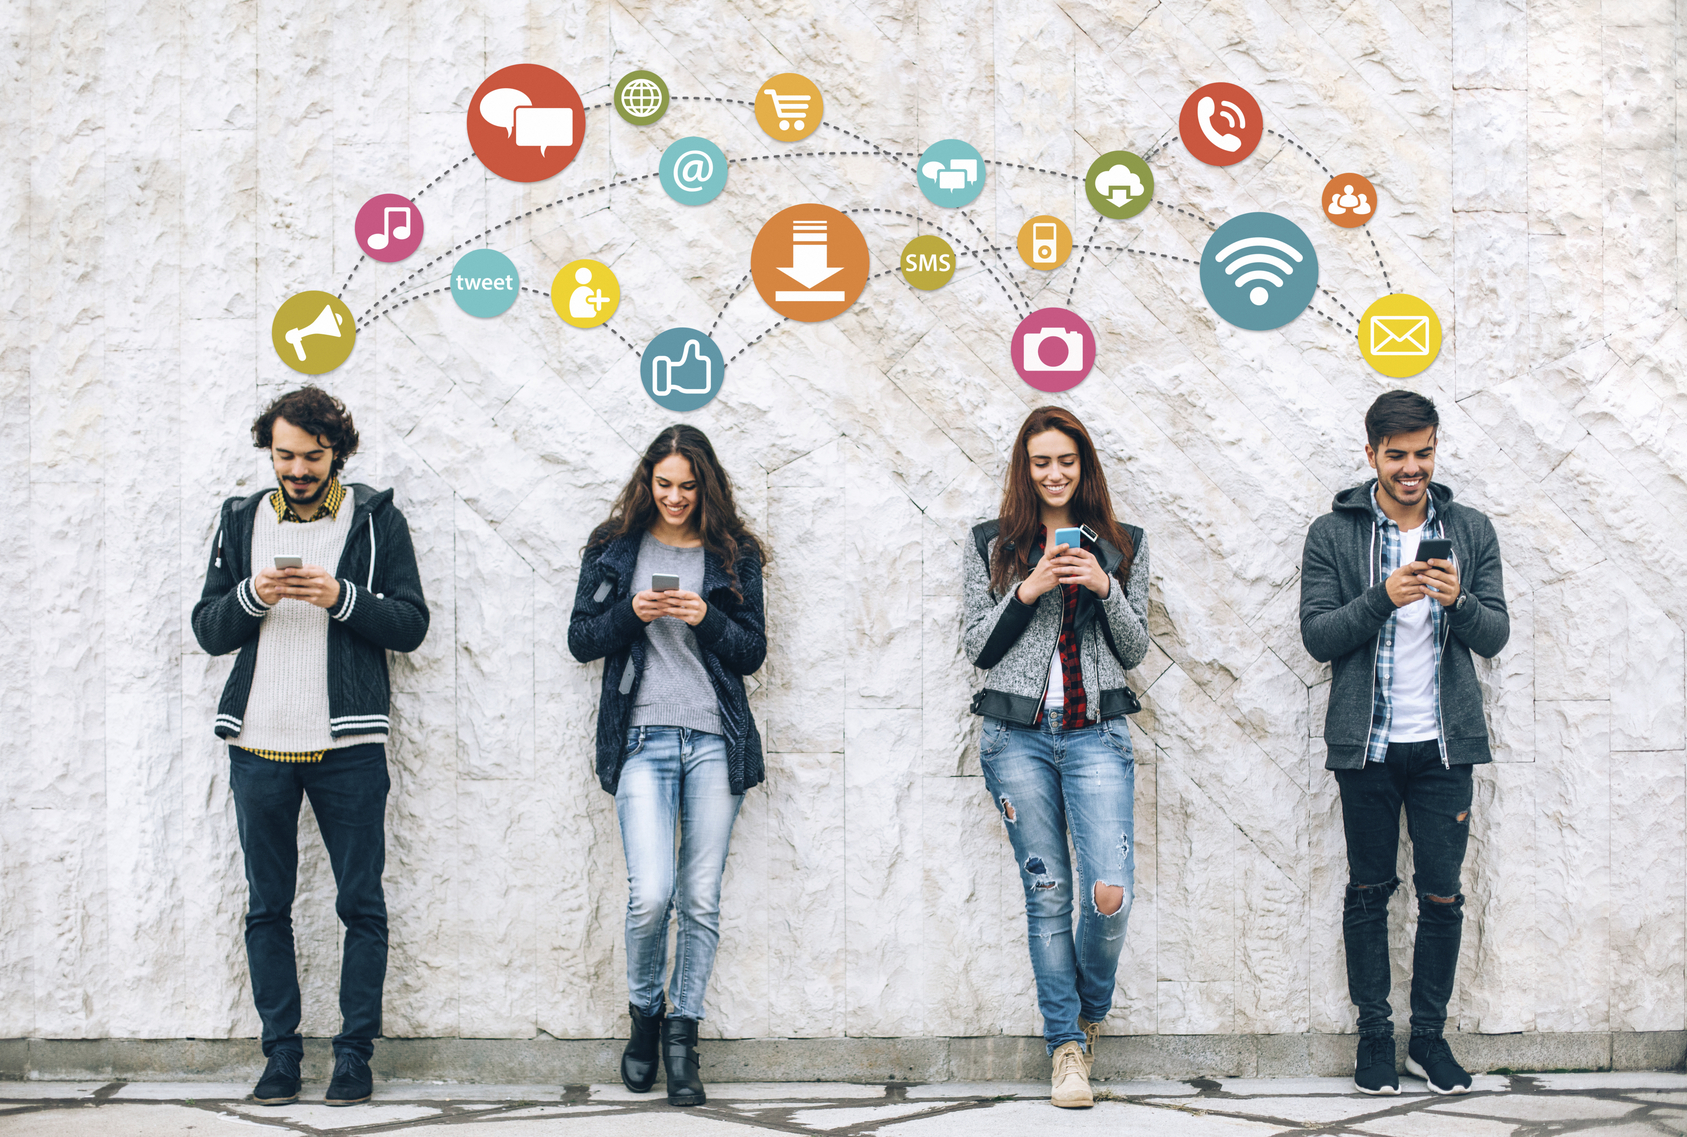
\includegraphics[width=\paperwidth,height=\paperheight]{images/competing_on_social_media.jpg}}
\begin{frame}{Cosa faremo}
    \vspace{0.8cm}
    \begin{block}{Siete Ragazze \textbf{Digitali}!}
      		\begin{itemize}
      		    \item Fake News
    			\item Social Network
    			\item Software Libero
    			\item Sicurezza
    		\end{itemize}
    \end{block}
\end{frame}

\setbeamertemplate{background}{}

\section{IDE}

\begin{frame}{IDE}
Un IDE (integrated development environment) e'

un programma con il quale programmiamo.

\vspace{3.0mm}
\begin{center}
    \href{https://www.jetbrains.com/pycharm-edu/download}{PyCharm Edu}
\end{center}
        
\begin{figure}
    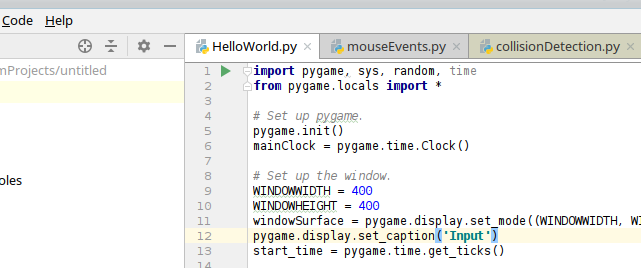
\includegraphics[height=5cm]{images/esempio_pycharm_editor.png}
\end{figure}

Avviamo il nostro programma cliccando sul triangolo verde nella linea 1
\end{frame}

\begin{frame}{IDE}
Un IDE (integrated development environment) e'

un programma con il quale programmiamo.
\vspace{4.0mm}
\begin{center}
    \href{https://www.spyder-ide.org/}{Spyder}
\end{center}

	\begin{columns}
		\begin{column}{3cm}
			\begin{figure}
   				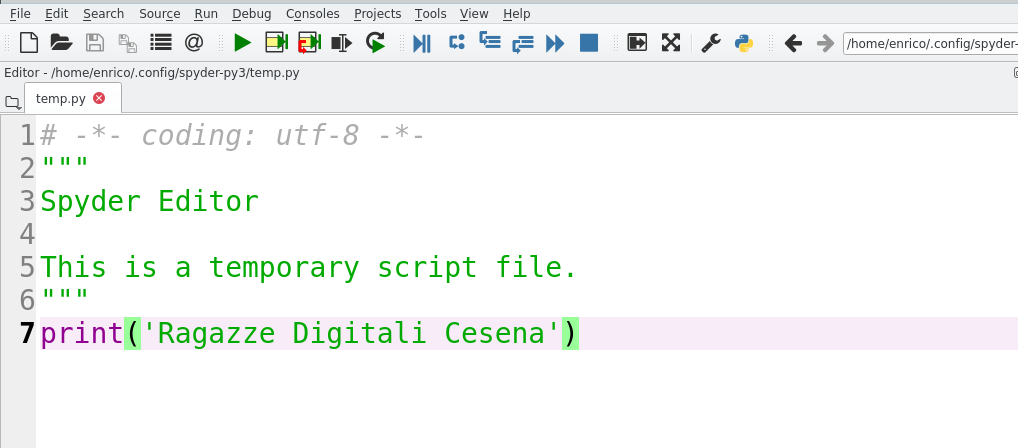
\includegraphics[height=5cm]{images/esempio_editor_spyder.png}
			\end{figure}
		\end{column}
		\begin{column}{6cm}
			\begin{figure}
   				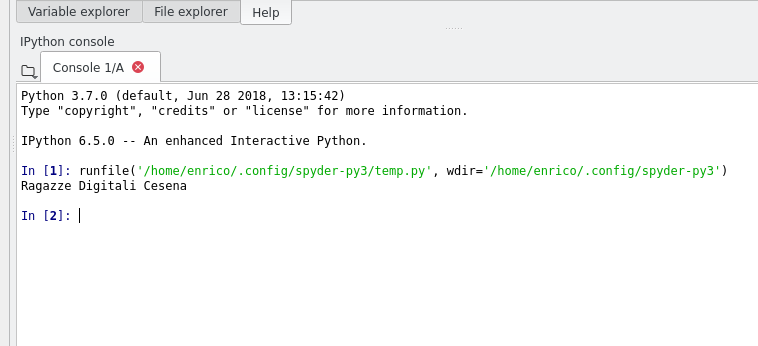
\includegraphics[height=5cm]{images/esempio_console_spyder.png}
			\end{figure}
		\end{column}
	\end{columns}
Avviamo il nostro programma cliccando sul triangolo verde in alto	
\end{frame}


\section{Operatori}

\begin{frame}{Iniziamo con qualche semplice operazione}
	\begin{columns}
		\begin{column}{4cm}
			\begin{figure}
   				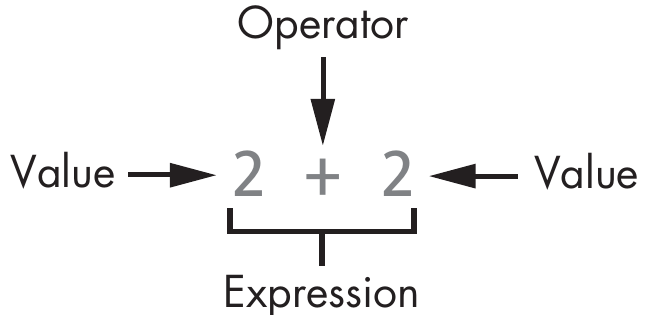
\includegraphics[height=2cm]{images/operatore_espressione.png}
			\end{figure}
		\end{column}
		\begin{column}{6cm}
            \begin{itemize}
                \item  6 + 6
                \item  7 - 5
                \item  8 / 4
                \item  9 * 3
                \item 12.5 * 3 cosa c'è di diverso qui?
                \item  (2 + 3 - 4) * 5 / 6 
            \end{itemize}
		\end{column}
	\end{columns}
\end{frame}

\begin{frame}{Iniziamo con qualche semplice operazione}
	\begin{columns}
		\begin{column}{4cm}
			\begin{figure}
   				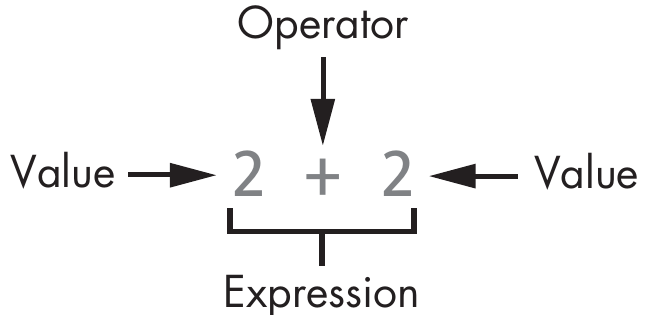
\includegraphics[height=2cm]{images/operatore_espressione.png}
			\end{figure}
		\end{column}
		\begin{column}{6cm}
            \begin{itemize}
                \item  6 + 6
                \item  7 - 5
                \item  8 / 4
                \item  9 * 3
                \item 12.5 * 3 cosa c'è di diverso qui?
                \item  (2 + 3 - 4) * 5 / 6 
            \end{itemize}
		\end{column}
	\end{columns}
	
	\begin{block}{Cosa succede se sbaglio a scrivere?}
	    5 +
	    
	    \lstinline{Syntax Error: Invalid syntax}
	\end{block}
\end{frame}

\section{Variabili}

\begin{frame}{}
	\begin{block}{Variabili}
        \begin{itemize}
            \item Le variabili sono "contenitori" di informazioni
            \item Posso \textbf{assegnare} un valore ad una variabile utilizzando il simbolo =
            \item Una variabile rappresenta un concetto - unico ma il cui valore può cambiare nel tempo
            
            Esempio:
                    
                    \lstinline{punti = 5}
            
                    accumulo punti e...
            
                    \lstinline{punti = 10}
            \item Dopo l'assegnamento non vedrò stampato nulla a video ma da quel momento la variabile "punti" avrà valore 10        
        \end{itemize}
	\end{block}

\end{frame}

\begin{frame}{Variabili}
    \begin{block}{Utilizziamo nomi ...}
        \begin{itemize}
            \item Significativi
            \item Pronunciabili
            \item Autoesplicativi
            \item Ricercabili (ad esempio è più facile cercare "cognome" rispetto a "cgnm")
            \item Che rappresentino un concetto
            \item Che appartengano al problema che si stà rappresentando
        \end{itemize}
    \end{block}
\end{frame}

%\begin{frame}{Variabili}
%    \begin{block}{"Il nostro codice deve essere...}
%        una piacevole lettura" [Cit. Prof. Mirko Viroli]
%    \end{block}
%\end{frame}

\begin{frame}
    \begin{block}{L'importanza di un buon nome per una variabile}
        \begin{itemize}
            \item Sembra facile ma non lo è.. ma fa risparmiare tempo e rende il nostro programma più comprensibile
            \item Se un nome richiede una spiegazione o un commento (che vedremo a breve) significa che non rivela il proprio intento.
            \item e = 15
            
            eta = 16
            \item
            b = 'sofia'
            
            nome = 'sofia'
        \end{itemize}
    \end{block}
\end{frame}

\begin{frame}{Variabili e Operatori}
    \begin{block}{Posso combinare tra loro variabili e operatori}
        \begin{itemize}
            \item anno = 2019
            
            anno = 2019 + 1
            \item
            anno = 2019
            
            annoDiNascita = 2005 
            
            eta = anno - annoDiNascita
            
            print(eta)
            \item e = 15
            
            eta = 16
            \item
            b = sofia
            
            nome = sofia
        \end{itemize}
    \end{block}
\end{frame}

\section{Testi}

\begin{frame}{Stringhe}
	\begin{block}{Chiameremo stringhe..}
        \begin{itemize}
            \item Testi
            \item Insieme di caratteri della tastiera
            
            ! qualsiasi carattere (lettere, numeri, punti, virgole, simboli ecc..)
        \end{itemize}

        \begin{figure}
            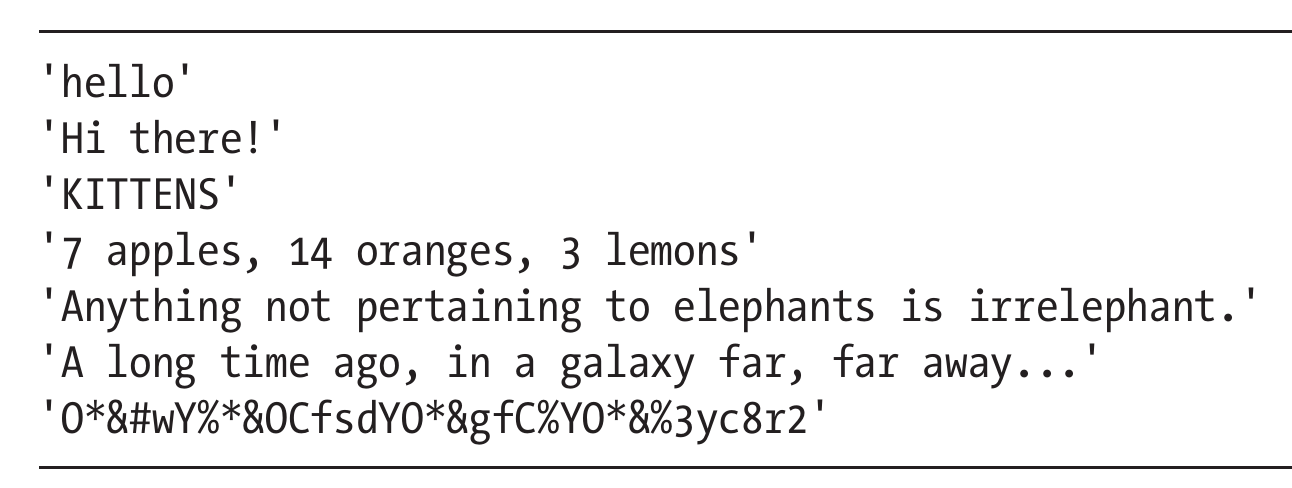
\includegraphics[height=3cm]{images/esempio_stringhe.png}
        \end{figure}
	\end{block}
	
	Notiamo negli esempi l'uso degli apici, all'interno dei quali viene scritta la stringa.
\end{frame}

\begin{frame}{Stringhe}
	\begin{block}{' ' oppure " " ?}
        \begin{itemize}
            \item Entrambi dicono a Python quando inizia e quando finisce una stringa
            \item Non ci sono particolari differenze, possiamo usarli come preferiamo.
            
            Ricordiamoci però di usare sempre lo stesso simbolo per l'inizio e la fine della stringa.
            
            'Ciao' OK
            
            \textbf{'}Ciao\textbf{"} NO
        \end{itemize}
	\end{block}
\end{frame}

\begin{frame}{Possiamo \textbf{concatenare} stringhe}
    \begin{itemize}
        \item 'Ciao ' + ' Ragazze Digitali'
        \item nome = 'Enrico'
            
        'Ciao ' + nome
        \item Ma non solo..
    \end{itemize}

	\begin{block}{Cosa succede se..}
        \begin{itemize}
            \item nome = Enrico
            
            \lstinline{NameError: name 'Enrico' is not defined}
            
            (Si aspetta una variabile di nome Enrico che non esiste, questo perchè non ho messo gli 'apici')
            \item 'Oggi siete in ' + numeroRagazzeSummerCamp
            
            \lstinline{TypeError: cannot concatenate 'str' and 'int' objects}
            
            Non posso concatenare stringhe con numeri, posso però convertire numeroRagazzeSummerCamp in stringa, vedremo come
        \end{itemize}
    \end{block}
\end{frame}

\section{Il nostro primo programma}

\begin{frame}[fragile]
\frametitle{Hello World}

    \begin{lstlisting}
print('Hello World')
# Qualsiasi testo preceduto dal cancelletto e' un commento
print('Come ti chiami?')
nome = input()
print('Benvenuta a Ragazze Digitali, ' + nome + '!')
    \end{lstlisting}

\end{frame}

\begin{frame}{Commenti}
        I commenti possono essere utili per spiegare parti di codice con il linuguaggio naturale.
        Python non esegue quello che c'è scritto in un commento ma lo ignora
\end{frame}

\begin{frame}

\begin{center}
    \bigskip
    Materiale rilasciato con licenza
    
    \textbf{\href{http://creativecommons.org/licenses/by-sa/4.0/}{Creative Commons - Attributions, Share-alike 4.0}}
    
    \medskip
    
\includegraphics[height=0.8cm]{images/cc.png}
\end{center}

\end{frame}


\end{document}
